\section{Convolution}
\begin{figure}
    \centering
    \begin{subfigure}{5cm}
        \centering
        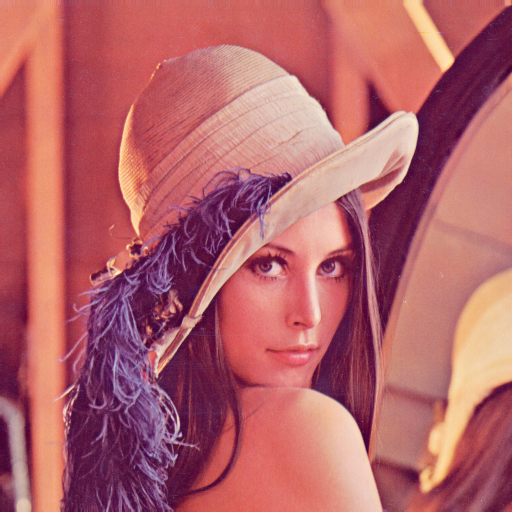
\includegraphics[width=4.5cm]{img/Lena}
        \caption{Original image}
    \end{subfigure}
    \begin{subfigure}{5cm}
        \centering
        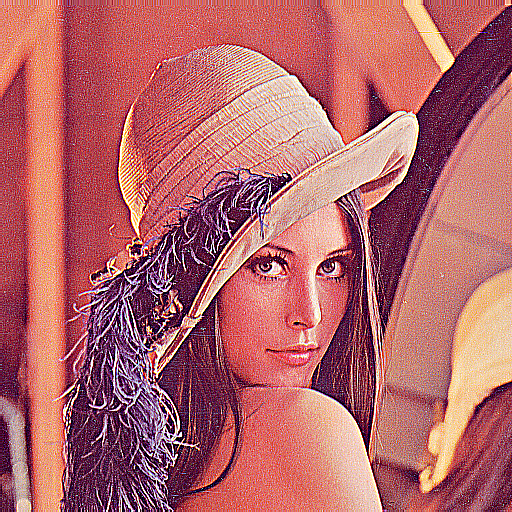
\includegraphics[width=4.5cm]{img/LenaProcessed}
        \caption{After sharpening}
    \end{subfigure}
    \caption{Lena test image}
    \label{fig:lena}
\end{figure}
\begin{figure}
    \centering
    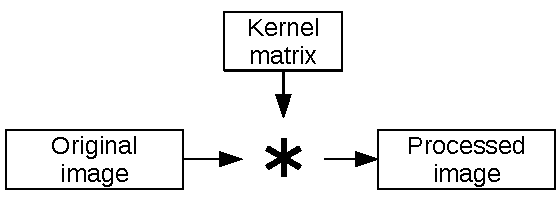
\includegraphics{img/BasicConvolution}
    \caption{Basic convolution in image processing}
    \label{fig:BasicConvolution}
\end{figure}

Convolution is a mathematical operation that can be applied to images or other signals in one or multiple dimensions.
This is commonly used by image processing software to produce blur, edge detect, sharpening filters and more.

An example of the result produced by a sharpening filter implemented with convolution can be seen in figure \ref{fig:lena}.
The convolution itself requires two inputs, the original image and a \textit{convolution kernel matrix}.
In the case of image processing, the kernel defines what kind of filter is applied.
The inputs and outputs of convolution when used for image processing is illustrated in figure \ref{fig:BasicConvolution}.
